\documentclass[11pt,aspectratio=169]{beamer}

\usepackage{rcstalk}
\usetheme{rcstheme}

\topic{Scheduling}
\subtitle{Lecture 10: Scheduling}

\begin{document}

\maketitle

\begin{slide}{CPU Scheduling}
%\centerline{
\hspace{2em}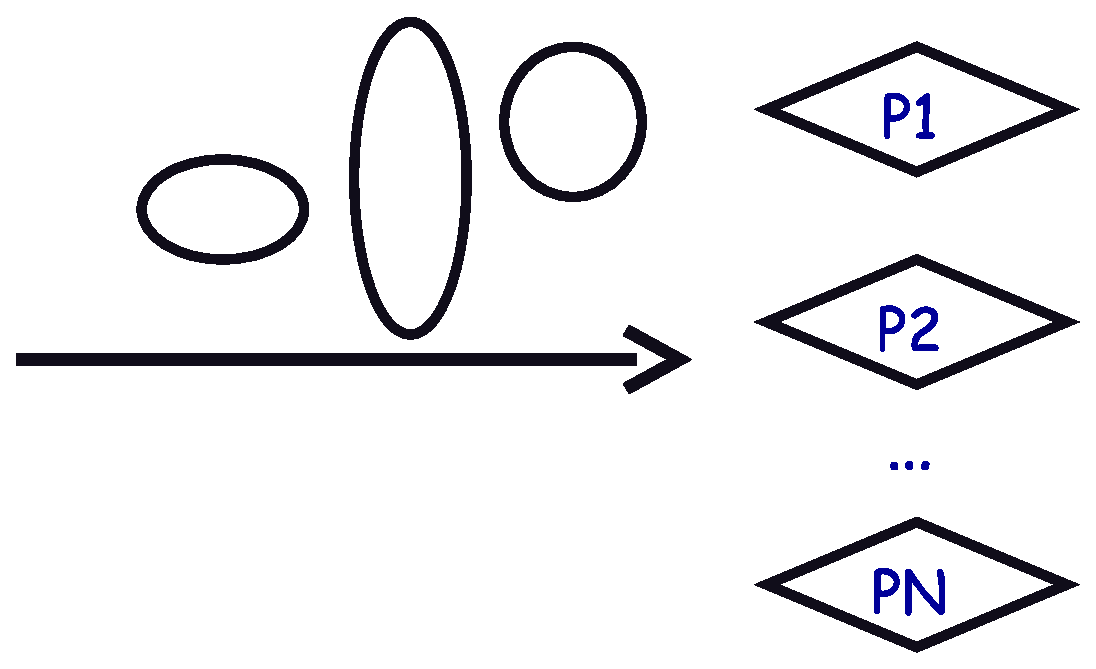
\includegraphics[width=3in]{figs/schedov}
\itms{
  \item The scheduling problem:
  \ittms{
  \item Have $K$ jobs ready to run
  \item Have $N\ge1$ CPUs
  \item Which jobs to assign to which CPU(s)
  }
  \item When do we make decision?
}
\end{slide}

\begin{slide}{CPU Scheduling}
\vspace{-1em}
%\centerline{
\hspace{2em}\includegraphics[width=3.7in]{procstate}
\itms{
  \item Scheduling decisions may take place when a process:
  \ittms{
    \item[1.] Switches from running to waiting state
    \item[2.] Switches from running to ready state
    \item[3.] Switches from new/waiting to ready
    \item[4.] Exits
  }
  \item Non-preemptive schedules use 1 \& 4 only
  \item Preemptive schedulers run at all four points
}
\end{slide}

\begin{slide}{Scheduling criteria}
\itms{
  \item Why do we care?
  \ittms{
    \item What goals should we have for a scheduling algorithm?
  }
\pause
\item \emph{Throughput} -- \# of procs that complete per unit time
\ittms{
  \item Higher is better
}
\item \emph{Turnaround time} -- time for each proc to complete
\ittms{
  \item Lower is better
}
\item \emph{Response time} -- time from request to first response \\
(e.g., key press to character echo, not launch to exit)
\ittms{
  \item Lower is better
}
\item Above criteria are affected by secondary criteria
\ittms{
  \item \emph{CPU utilization} -- fraction of time CPU doing productive work
  \item \emph{Waiting time} -- time each proc waits in ready queue
}
}
\end{slide}

\begin{slide}{Example: FCFS Scheduling}
\itms{
  \item Run jobs in order that they arrive
  \ittms{
    \item Called ``\emph{First-come first-served}'' (FCFS)
    \item E.g.., Say $P_1$ needs 24 sec, while $P_2$ and $P_3$ need 3.
    \item Say $P_2$, $P_3$ arrived immediately after $P_1$, get: \\[4pt]
     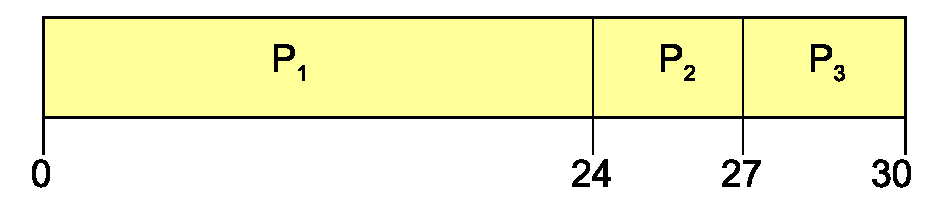
\includegraphics[width=3.3in]{figs/fcfs1}
  }
  \item Dirt simple to implement---how good is it?
  \item Throughput: 3 jobs / 30 sec = 0.1 jobs/sec
  \item Turnaround Time: $P_1: 24$, $P_2: 27$, $P_3: 30$
  \ittms{
    \item Average TT: $(24+27+30)/3=27$
  }
  \item Can we do better?
}
\end{slide}

\begin{slide}{FCFS continued}
\itms{
  \item Suppose we scheduled $P_2$, $P_3$, then $P_1$
  \ittms{
    \item Would get:\\[4pt]
     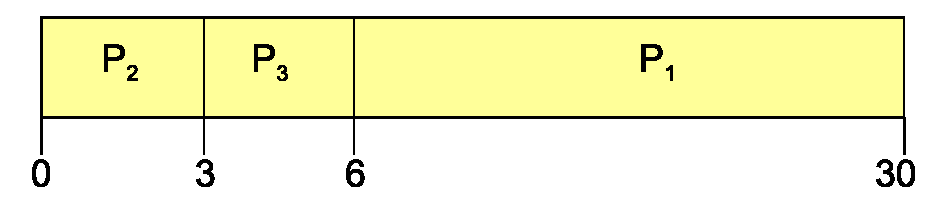
\includegraphics[width=3.3in]{figs/fcfs2}
  }
  \item Throughput: 3 jobs / 30 sec = 0.1 jobs/sec
  \item Turnaround time: $P_1: 30$, $P_2: 3$, $P_3: 6$
  \ittms{
    \item Average TT: $(30+3+6)/3=13$ -- much less than 27
  }
  \item Lesson: scheduling algorithm can reduce TT
  \ittms{
    \item Minimizing waiting time can improve RT and TT
  }
  \item What about throughput?
}
\end{slide}

\begin{slide}{View CPU and I/O devices the same}
\itms{
  \item CPU is one of several devices needed by users' jobs
  %\item An I/O device is like a special-purpose CPU
  \ittms{
    \item CPU runs compute jobs, Disk drive runs disk jobs, etc.
    \item With network, part of job may run on remote CPU
%    \item ``special purpose'' = disk drive can only run a disk job, tape
%      drive a tape job, \ldots
  }
  \item Scheduling 1-CPU system with $n$ I/O devices like scheduling
    asymmetric $(n+1)$-CPU multiprocessor
  \ittms{
    \item Result: all I/O devices + CPU busy $\rightarrow$ n+1 fold
      speedup! \\[2mm]
      %\centerline{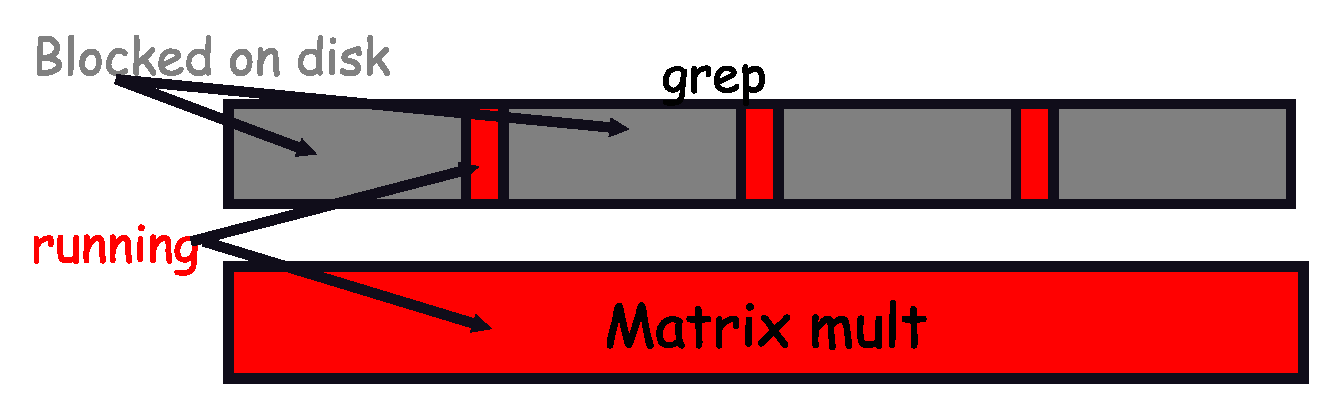
\includegraphics[width=4.0in]{figs/iocpu}}
      \centerline{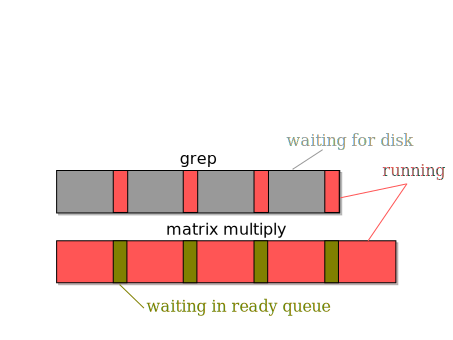
\includegraphics[width=80mm]{overlap}}
    \item Overlap them just right?  throughput will be almost doubled
  }
}
\end{slide}

\begin{frame}
\frametitle{Bursts of computation \& I/O}
\begin{columns}
\column{72mm}
\itms{
  \item Jobs contain I/O and computation
  \ittms{
    \item Bursts of computation
    \item Then must wait for I/O
  }
  \item To Maximize throughput
  \ittms{
    \item Must maximize CPU utilization
    \item Also maximize I/O device utilization
  }
  \item How to do?
  \ittms{
    \item Overlap I/O \& computation from multiple jobs
    \item \Red{Means \emph{response time} very important for I/O-intensive
      jobs:}  I/O device will be idle until job gets small amount of CPU
      to issue next I/O request
  }
}
\column{0mm}
\column{42mm}
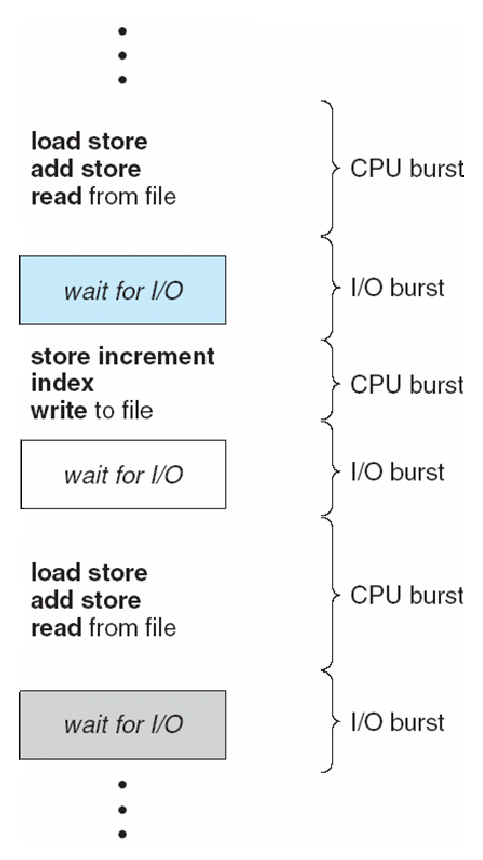
\includegraphics[width=42mm]{figs/bursts}
\end{columns}
\end{frame}

\begin{slide}{Histogram of CPU-burst times}
\centerline{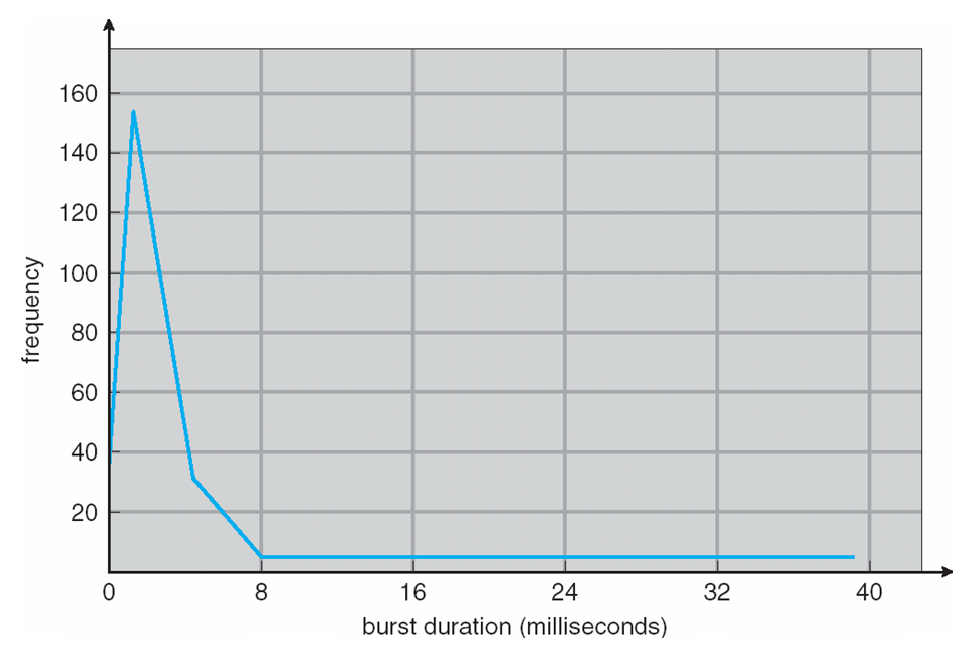
\includegraphics[height=2.7in]{figs/bursthist}}
\itms{
  \item What does this mean for FCFS?
}
\end{slide}

\begin{slide}{FCFS Convoy effect}
\itms{
  \item CPU-bound jobs will hold CPU until exit or I/O \\
      (but I/O rare for CPU-bound thread)
\ittms{
  \item long periods where no I/O requests issued, and CPU held
  \item Result: poor I/O device utilization
}
\item Example: one CPU-bound job, many I/O bound
\ittms{
\item CPU-bound job runs (I/O devices idle)
\item CPU-bound job blocks
\item I/O-bound job(s) run, quickly block on I/O
\item CPU-bound job runs again
\item I/O completes
\item CPU-bound job continues while I/O devices idle
}
\item Simple hack: run process whose I/O completed?
\ittms{
\item What is a potential problem?
}}
\end{slide}

\begin{slide}{SJF Scheduling}
\itms{
  \item \emph{Shortest-job first} (SJF) attempts to minimize TT
  \ittms{
    \item Schedule the job whose next CPU burst is the shortest
  }
  \item Two schemes:
  \ittms{

    \item \emph{Non-preemptive} -- once CPU given to the process it
    cannot be preempted until completes its CPU burst

    \item \emph{Preemptive} -- if a new process arrives with CPU burst
length less than remaining time of current executing process, preempt
(Known as the \emph{Shortest-Remaining-Time-First} or SRTF)

  }
\item What does SJF optimize?
\pause
\ittms{
 \item Gives minimum average \emph{waiting time} for a given set of
   processes
}
}
\end{slide}

\begin{slide}{Examples}
\centerline{\small
    \begin{tabular}{ccc}
        Process	& Arrival Time	& Burst Time \\
        $P_1$	& 0.0	& 7 \\
        $P_2$	& 2.0	& 4 \\
        $P_3$	& 4.0	& 1 \\
        $P_4$	& 5.0	& 4 \\
\end{tabular}}
\itms{
  \item Non-preemptive \\
    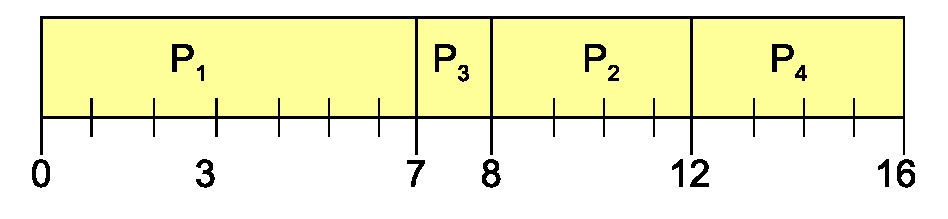
\includegraphics[width=3.3in]{figs/sjfnp}
  \item Preemptive \\
    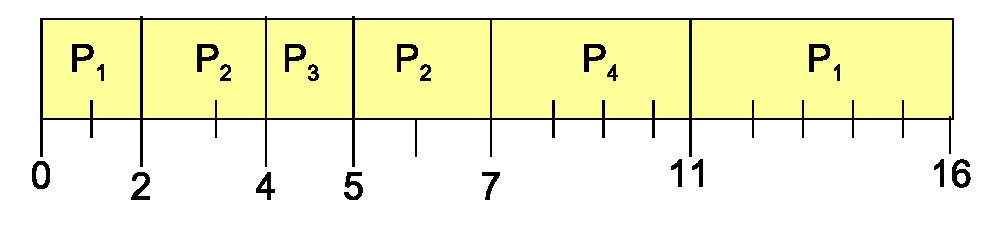
\includegraphics[width=3.3in]{figs/sjfp}
  \item Drawbacks?
}
\end{slide}

\begin{slide}{\only<2>{\hypertarget{sjf-limitations}}SJF limitations}
\itms{
  \item Doesn't always minimize average turnaround time
  \ittms{
    \item Only minimizes waiting time, which minimizes response time
    \item Example where turnaround time might be suboptimal?
    \onslide<2->{\item Overall longer job has shorter bursts}
  }
  \item Can lead to unfairness or starvation
  \item In practice, can't actually predict the future
  \item But can estimate CPU burst length based on past
  \ittms{
    \item Exponentially weighted average a good idea
    \item $t_n$ actual length of proc's $n^\mathrm{th}$ CPU burst
    \item $\tau_{n+1}$ estimated length of proc's $n+1^\mathrm{st}$
    \item Choose parameter $\alpha$ where $0<\alpha\le1$
    \item Let $\tau_{n+1}=\alpha t_n+(1-\alpha)\tau_n$
  }
}
\end{slide}

\begin{slide}{Exp. weighted average example}
\centerline{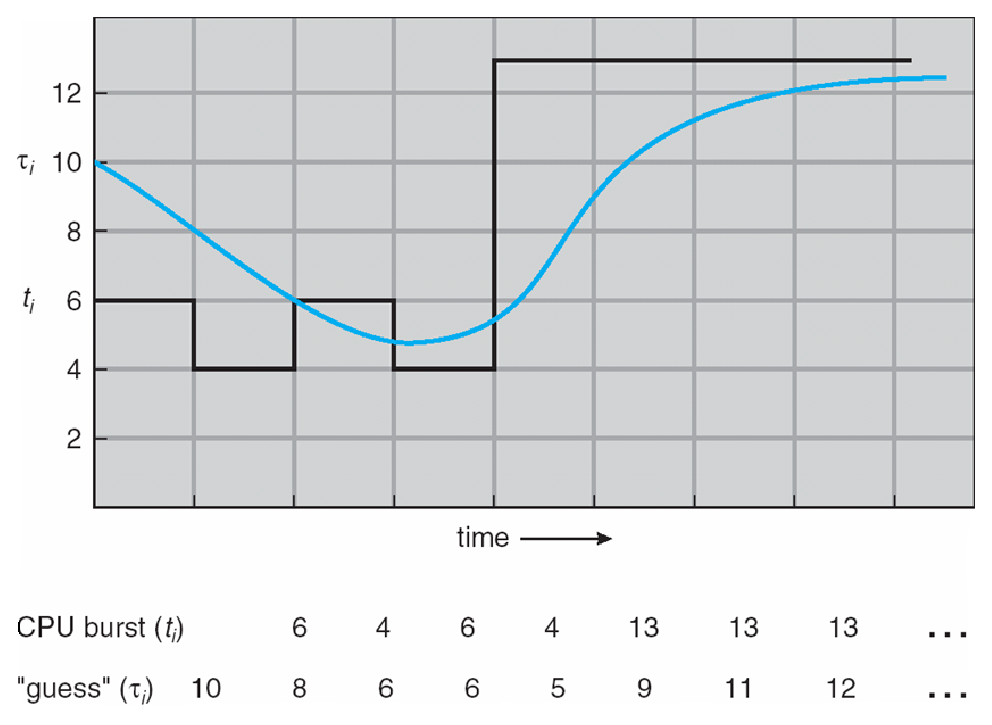
\includegraphics[width=4in]{figs/predict}}
\end{slide}

\begin{slide}{Round robin (RR) scheduling}
\centerline{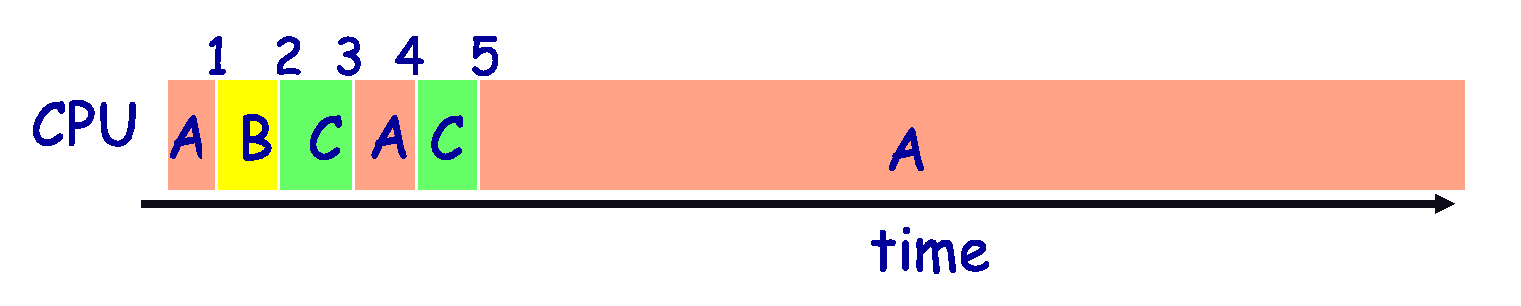
\includegraphics[width=3.3in]{figs/rr}}
\itms{
  \item Solution to fairness and starvation
  \ittms{
    \item Preempt job after some time slice or \emph{quantum}
    \item When preempted, move to back of FIFO queue
    \item (Most systems do some flavor of this)
  }
  \item Advantages:
  \ittms{
    \item Fair allocation of CPU across jobs
    \item Low average waiting time when job lengths vary
    \item Good for responsiveness if small number of jobs
  }
  \item Disadvantages?
}
\end{slide}

\begin{slide}{RR disadvantages}
\itms{
  \item Varying sized jobs are good 
    \ldots what about same-sized jobs?
  \item  Assume 2 jobs of time=100 each: \\
\centerline{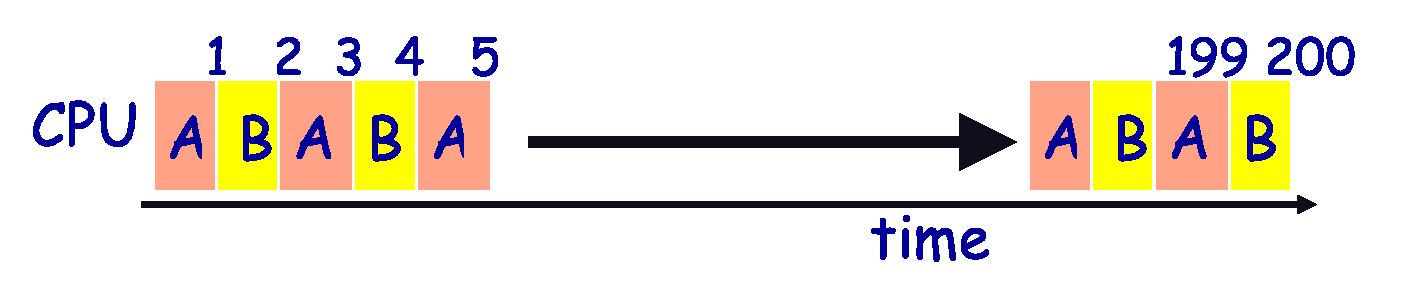
\includegraphics[width=3.3in]{figs/rrbad}}
  \item Even if context switches were free\ldots
  \ittms{
    \item What would average completion time be with RR?
      \onslide<2>{\emph{199.5}}
    \item How does that compare to FCFS?   \onslide<2>{\emph{150}}
  }
}
\end{slide}

\begin{slide}{Context switch costs}
\itms{
  \item What is the cost of a context switch?
\pause
  \item Brute CPU time cost in kernel
  \ittms{
      \item Save and restore resisters, etc.
      \item Switch address spaces (expensive instructions)
  }
  \item Indirect costs: cache, buffer cache, \& TLB misses
}
\onslide<2->
\centerline{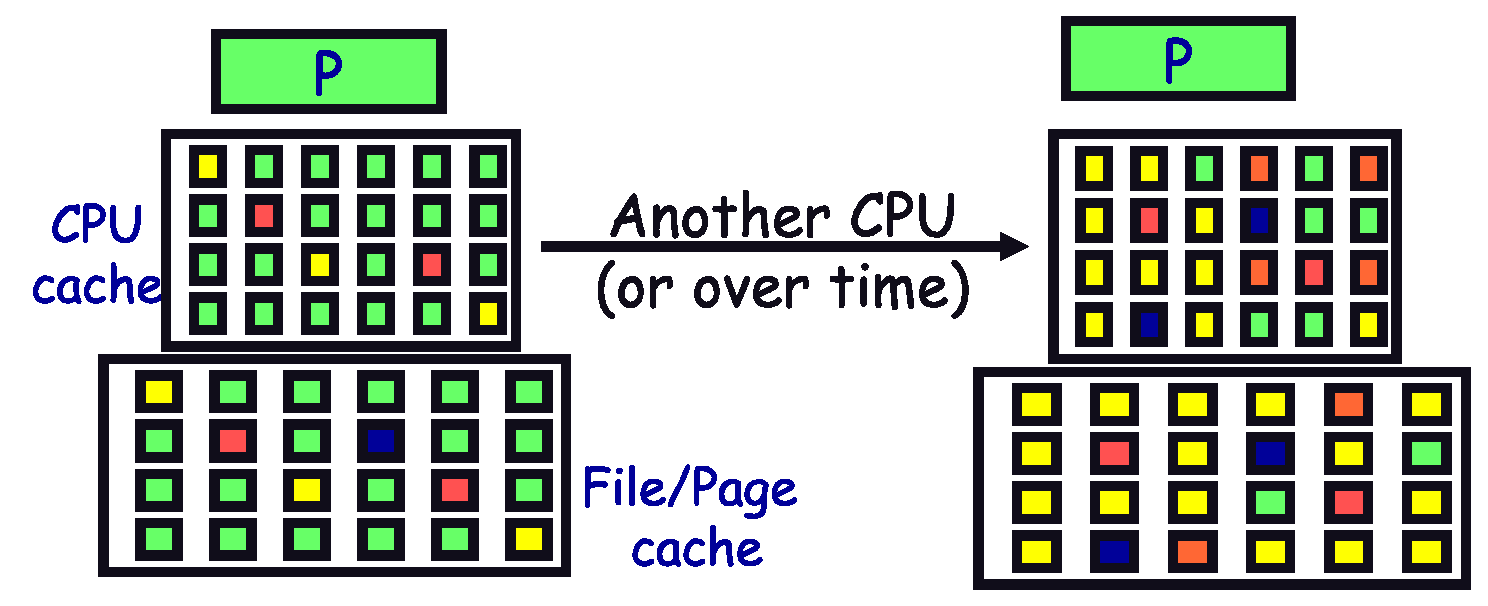
\includegraphics[height=1.7in]{figs/cswitch-cost}}
\end{slide}

\begin{slide}{Time quantum}
\centerline{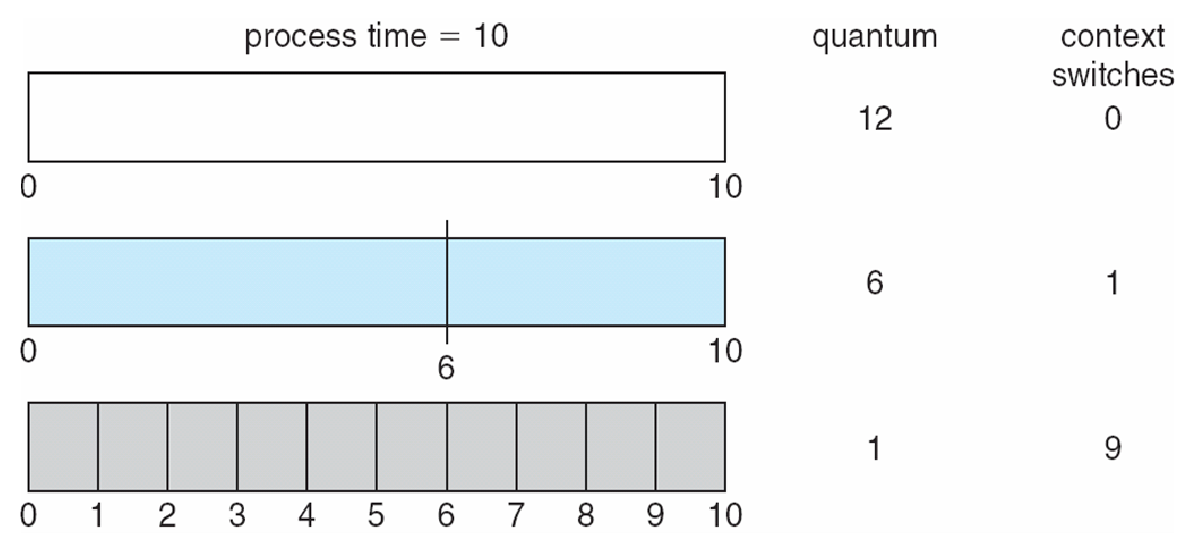
\includegraphics[width=96mm]{figs/quantum}}

\itms{
  \item How to pick quantum?
  \ittms{
    \item Want much larger than context switch cost
    \item Majority of bursts should be less than quantum
    \item But not so large system reverts to FCFS
  }
  \item Typical values: 10--100 msec
}
\end{slide}

\begin{slide}{Turnaround time vs.\ quantum}
\centerline{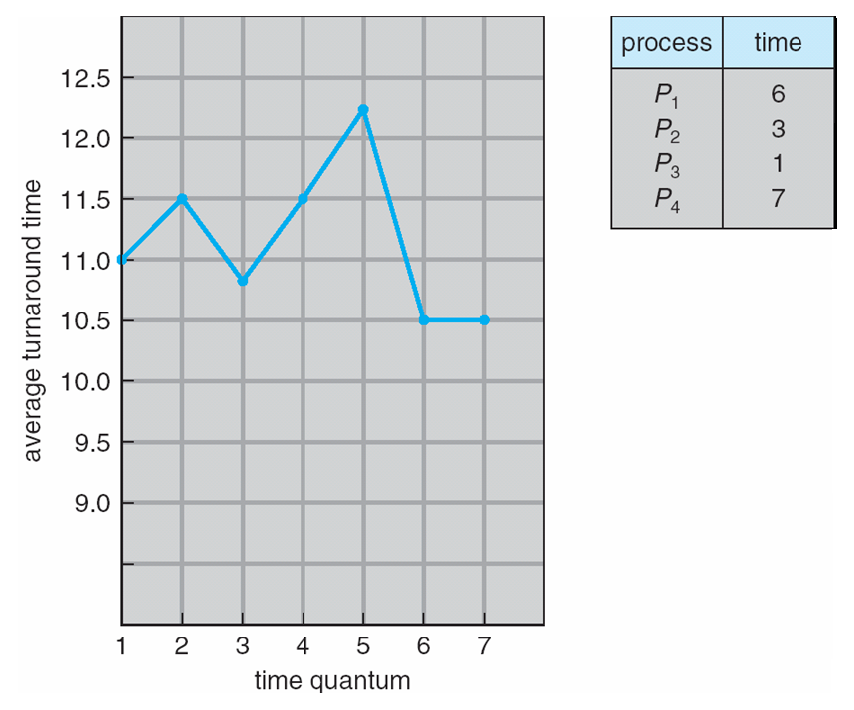
\includegraphics[height=3in]{figs/tt-vs-q}}
\end{slide}

\begin{slide}{Two-level scheduling}
\itms{
  \item Switching to swapped out process very expensive
  \ittms{
    \item Swapped out process has most memory pages on disk
    \item Will have to fault them all in while running
    \item One disk access costs $\sim$10ms.  On 1GHz machine, 10ms = 10
      million cycles!
  }
  \item Context-switch-cost aware scheduling
  \ittms{
    \item Run in-core subset for ``a while''
    \item Then swap some between disk and memory
  }
  \item How to pick subset?  How to define ``a while''?
  \ittms{
    \item View as scheduling \emph{memory} before scheduling CPU
    \item Swapping in process is cost of memory ``context switch''
    \item So want ``memory quantum'' much larger than swapping cost
  }
}
\end{slide}

\begin{slide}{Priority scheduling}
\itms{
\item  Associate a numeric priority with each process
\ittms{
  \item E.g., smaller number means higher priority (Unix/BSD)
}
\item Give CPU to the process with highest priority
\ittms{
  \item Can be done preemptively or non-preemptively
}
\item Note SJF is a priority scheduling where priority is the predicted next CPU burst time
\item Starvation -- low priority processes may never execute
\item Solution?
\onslide<2->
\ittms{
\item Aging: increase a process's priority as it waits
}}
\end{slide}


\begin{slide}{Multilevel feeedback queues (BSD)}
\centerline{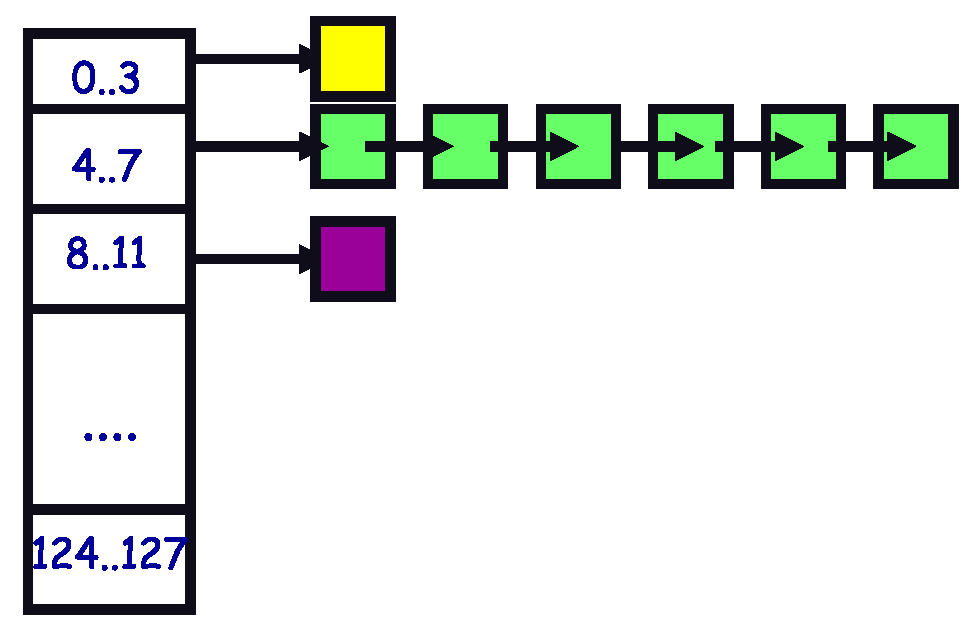
\includegraphics[height=1.5in]{figs/bsd}}
\itms{
  \item Every runnable process on one of 32 run queues
  \ittms{
    \item Kernel runs process on highest-priority non-empty queue
    \item Round-robins among processes on same queue
  }
  \item Process priorities dynamically computed
  \ittms{
    \item Processes moved between queues to reflect priority changes
    \item If a process gets higher priority than running process, run it
  }
  \item Idea:  Favor interactive jobs that use less CPU
}
\end{slide}

\begin{slide}{Process priority}
\itms{
  \item \Red{\texttt{p\_nice}} -- user-settable weighting factor
  \item \Red{\texttt{p\_estcpu}} -- per-process estimated CPU usage
  \ittms{
    \item Incremented whenever timer interrupt found proc.\ running
    \item Decayed every second while process runnable
\[ \mathtt{p\_estcpu} \gets \left({2\cdot\mathrm{load}\over
        2\cdot\mathrm{load}+1}\right)\mathtt{p\_estcpu} + \mathtt{p\_nice} \]
    \item Load is sampled average of length of run queue plus short-term
      sleep queue over last minute
  }
  \item Run queue determined by $\mathtt{p\_usrpri}/4$
\[ \mathtt{p\_usrpri} \gets 50 + \left({\mathtt{p\_estcpu}\over
        4}\right) + 2 \cdot \mathtt{p\_nice} \]
(value clipped if over 127)
}
\end{slide}

\begin{slide}{Sleeping process increases priority}
%\vspace*{-.2in}
\itms{
  \item \texttt{p\_estcpu} not updated while asleep
  \ittms{
    \item Instead \texttt{p\_slptime} keeps count of sleep time
  }
  \item When process becomes runnable
\[ \mathtt{p\_estcpu} \gets \left({2\cdot\mathrm{load}\over
  2\cdot\mathrm{load}+1}\right)^{\mathtt{p\_slptime}}\times\mathtt{p\_estcpu}
\]
  \ittms{
    \item Approximates decay ignoring nice and past loads
  }
  \item Previous description based on {\em The Design and Implementation of the 
      4.4BSD Operating System} by McKusick
}
\vspace*{.1in}
\end{slide}

%% \begin{slide}{Limitations of BSD scheduler}
%% \itms{
%%   \item Hard to have isolation / prevent interference (e.g.,
%%     w. vservers)
%%   \ittms{
%%     \item Priorities are absolute
%%   }
%%   \item Can't donate priority (e.g., to server on RPC)
%%   \item No flexible control
%%   \ittms{
%%     \item E.g., In monte carlo simulations, error is $1/\sqrt{N}$ after
%%       $N$ trials
%%     \item Want to get quick estimate from new computation
%%     \item Leave a bunch running for a while to get more accurate results
%%   }
%%   \item Multimedia applications
%%   \ittms{
%%     \item Often fall back to degraded quality levels depending on resources
%%     \item Want to control quality of different streams
%%   }
%% }
%% \end{slide}

%% \begin{slide}{Process scheduling}
%% \itms{
%%   \item Goal:  High throughput
%%   \ittms{
%%     \item Minimize context switches to avoid wasting CPU, TLB misses,
%%         cache misses, even page faults.
%%   }
%%   \item Goal:  Low latency
%%   \ittms{
%%     \item People typing at editors want fast response
%%     \item Network services can be latency-bound, not CPU-bound
%%   }
%%   \item BSD time quantum:  $1/10$~sec (since $\sim$1980)
%%   \ittms{
%%     \item Empirically longest tolerable latency
%%     \item Computers now faster, but job queues also shorter
%%   }
%%   \item Solaris SVR4: $1/100$~sec
%% }
%% \end{slide}

%% \begin{slide}{Scheduling algorithms}
%% \itms{
%%   \item Round-robin
%%   \item Priority scheduling
%%   \item Shortest process next (if you can estimate it)
%%   \item Fair-Share Schedule (try to be fair at level of users, not
%%     processes)
%%   \item Fancy combinations of the above (e.g., SMART)
%% }
%% \end{slide}

%  \begin{slide}{Real-time scheduling}
%  \itms{
%    \item Two categories:
%    \ittms{
%      \item \emph{Soft real time}---miss deadline and CD will sound funny
%      \item \emph{Hard real time}---miss deadline and plane will crash
%    }
%    \item System must handle periodic and aperiodic events
%    \ittms{
%      \item E.g., procs A, B, C must be scheduled every 100, 200, 500~msec,
%        require 50, 30, 100 msec respectively
%      \item \emph{Schedulable} if $\displaystyle\sum {CPU\over
%  	  \mathrm{period}} \le 1$ (not counting switch time)
%    }
%    \item Variety of scheduling strategies
%    \ittms{
%      \item E.g., first deadline first \\
%        (works if schedulable, otherwise fails spectacularly)
%    }
%  }
%  \end{slide}

\begin{slide}{Multiprocessor scheduling issues}
%\vspace*{-.1in}
\itms{
  \item Must decide on more than which processes to run
  \ittms{
    \item Must decide on which CPU to run which process
  }
  \item Moving between CPUs has costs
  \ittms{
    \item More cache misses, depending on arch more TLB misses too
  }
  \item \emph{Affinity scheduling}---try to keep threads on same CPU
}
\centerline{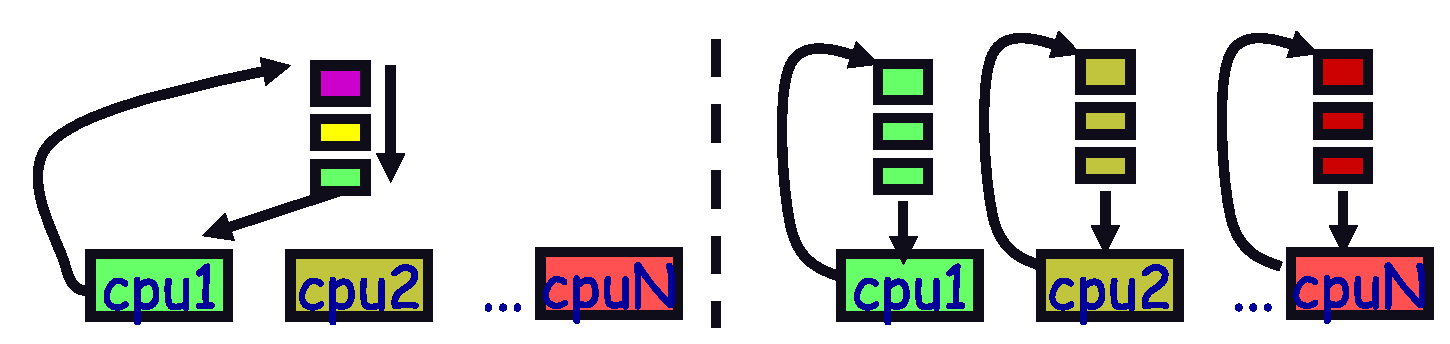
\includegraphics[width=3.5in]{figs/affinity}}
\itms{
  \item[]
  \ittms{
    \item But also prevent load imbalances
    \item Do \emph{cost-benefit} analysis when deciding to migrate
  }
}
\end{slide}

\begin{slide}{Multiprocessor scheduling (cont)}
\itms{
  \item Want related processes scheduled together
  \ittms{
    \item Good if threads access same resources (e.g., cached files)
    \item Even more important if threads communicate often, \\
      otherwise must context switch to communicate
  }
  \item \emph{Gang scheduling}---schedule all CPUs synchronously
  \ittms{
    \item With synchronized quanta, easier to schedule related
       processes/threads together
  }
\centerline{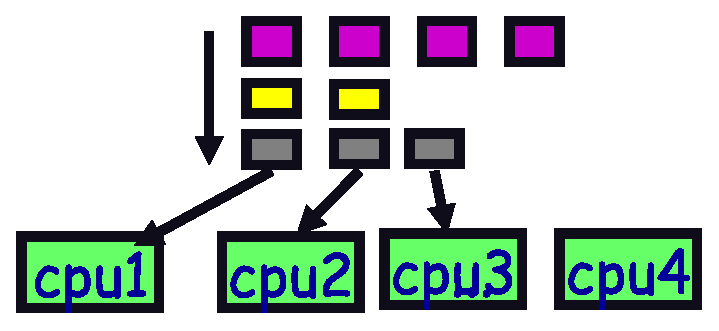
\includegraphics[width=3in]{figs/gang}}
}
\end{slide}

% \begin{slide}{Thread scheduling}
% \itms{
% \item With thread library, have two scheduling decisions:
% \ittms{
% \item \emph{Local Scheduling} -- Thread library decides which
% user thread to put onto an available kernel thread
% 
% \item \emph{Global Scheduling} -- Kernel decides which kernel
% thread to run next
% }
% \item Can expose to the user
% \ittms{
%   \item E.g., \texttt{pthread\_attr\_setscope} allows two choices
%   \item \texttt{PTHREAD\_SCOPE\_SYSTEM} -- thread scheduled like a
%   process (effectively one kernel thread bound to user thread 
%   -- Will return ENOTSUP in user-level pthreads implementation)
%   \item \texttt{PTHREAD\_SCOPE\_PROCESS} -- thread scheduled within
%     the current process (may have multiple user threads multiplexed
%     onto kernel threads)
% }
% }
% \end{slide}

\begin{slide}{Thread dependencies}
\itms{
  \item Say $H$ at high priority, $L$ at low priority
  \ittms{
    \item $L$ acquires lock $l$.
    \item Scenario 1: $H$ tries to acquire $l$, fails, spins.  $L$
      never gets to run.
    \item Scenario 2: $H$ tries to acquire $l$, fails, blocks. $M$
      enters system at medium priority.  $L$ never gets to run.
    \item Both scenes are examples of \Red{\emph{priority inversion}}
  }
  \item Scheduling = deciding who should make progress
  \ittms{
    \item A thread's importance should increase with the importance of
      those that depend on it
    \item Na\"\i ve priority schemes violate this
  }
}
\end{slide}

\begin{slide}{Priority donation}
\itms{
  \item Example 1: $L$ low, $M$ medium, $H$ high priority
  \ittms{
    \item $L$ holds lock $l$
    \item $M$ waits on $l$, $L$'s priority raised to $L_1 =
      \max(M, L) = 4$
    \item Then $H$ waits on $l$, $L$'s priority raised to $\max(H, L_1)
      = 8$
  }
  \item Example 2: Same $L, M, H$ as above
  \ittms{
    \item $L$ holds lock $l$, $M$ holds lock $l_2$
    \item $M$ waits on $l$, $L$'s priority now $L_1=4$ (as before)
    \item Then $H$ waits on $l_2$.  $M$'s priority goes to $M_1=\max(H,
      M)=8$, \emph{and} $L$'s priority raised to $\max(M_1, L_1)=8$
  }
  \item Example 3: $L$ (prio 2), $M_1, \ldots M_{1000}$ (all prio 4)
  \ittms{
    \item $L$ has $l$, and $M_1, \ldots, M_{1000}$ all block on $l$.
      $L$'s priority is $\max(L, M_1, \ldots, M_{1000})=4$.
  }
}
\end{slide}


\begin{slide}{Borrowed Virtual Time Scheduler \cref{readings/bvt.pdf}{[Duda]}}
\itms{
  \item Many modern schedulers employ notion of \emph{virtual time}
  \begin{itemize}
    \item Idea: Equalize virtual CPU time consumed by different
      processes
    \item Examples: Linux CFS
  \end{itemize}
%  \ittms{
%    \item Algorithm proposed by Duda \& Cheriton in 1999
%  }
  %% \item Goals:
  %% \ittms{
  %%   \item Support mix of soft real-time and best-effort tasks
  %%   \item Simple to use (avoid 1,000,000 knobs to tweak)
  %%   \item Should be easy, efficient to implement
  %% }
  \item Idea:  Run process w.\ lowest \emph{effective virtual time}
  \ittms{
    \item $A_i$ -- \emph{actual virtual time} consumed by process $i$
    \item \emph{effective virtual time} $E_i = A_i - (\mathrm{warp}_i
  \mathrel{?} W_i \mathrel{:} 0)$
  }
  \item Supports real-time applications:
  \ittms{
    \item Warp factor allows borrowing against future CPU time
    \item Allows an application to temporarily violate fairness
%  \\ \ldots hence name of algorithm

  }
}
\end{slide}

\begin{slide}{Process weights}
\itms{
  \item Each process $i$'s faction of CPU determined by weight $w_i$
  \ittms{
    \item $i$ should get $w_i/\sum\limits_j w_j$ faction of CPU
    \item So $w_i$ is seconds per virtual time tick while $i$ has CPU
  }
  \item When $i$ consumes $t$ CPU time,
    track it:  $A_i\mathrel{\texttt{+=}}t/w_i$
%  \ittms{
%    \item As with stride, pick some large $N$ (like $\mathrm{stride}_1$)
%    \item Pre-compute $m_i=N/w_i$, then set
%  $A_i\mathrel{\texttt{+=}}t\cdot m_i$
%  }
  \item Example:  gcc (weight 2), bigsim (weight 1)
  \ittms{
    \item Assuming no IO, runs: gcc, gcc, bigsim, gcc, gcc, bigsim, \ldots
    \item Lots of context switches, not so good for performance
  }
  \item Add in context switch allowance, $C$
  \ittms{
    \item Only switch from $i$ to $j$ if $E_j\le E_i-C/w_i$
    \item $C$ is wall-clock time ($>\!\!>$ context switch cost), so must
      divide by $w_i$
    \item Ignore $C$ if $j$ just became runable%
      \only<1>{\ldots why?}\only<2>{ to avoid affecting response time}
  }
}
\end{slide}

\begin{slide}{BVT example}
\centerline{\hspace*{-.3in}\input{bvt1}}
\itms{
  \item gcc has weight 2, bigsim weight 1, $C=2$, no I/O
  \ittms{
    \item bigsim consumes virtual time at twice the rate of gcc
%\item Procs always run for $C$ time after exceeding other's
%     $E_i$
  }
}
\end{slide}

\begin{slide}{Sleep/wakeup}
\itms{
  \item Must lower priority (increase $A_i$) after wakeup
  \ittms{
    \item Otherwise process with very low $A_i$ would starve everyone
  }
  \item Bound lag with Scheduler Virtual Time (SVT)
  \ittms{
    \item SVT is minimum $A_j$ for all runnable threads $j$
    \item When waking $i$ from voluntary sleep, set
      $A_i\gets\max(A_i,SVT)$
  }
  \item Note voluntary/involuntary sleep distinction
  \ittms{
    \item E.g., Don't reset $A_j$ to SVT after page fault
    \item Faulting thread needs a chance to catch up
    \item But do set $A_i\gets\max(A_i,SVT)$ after socket read
  }
  \item Note: Even with SVT \Red{$A_i$ can never decrease}
  \ittms{
    \item After short sleep, might have $A_i>\mathrm{SVT}$, so
  $\max(A_i,SVT)=A_i$ 
    \item $i$ never gets more than its fair share of CPU in long run
  }
}
\end{slide}

\begin{slide}{gcc wakes up after I/O}
\centerline{\input{bvt2}}
\itms{
  \item gcc's $A_i$ gets reset to SVT on wakeup
  \ittms{
    \item Otherwise, would be at lower (blue) line and starve bigsim
  }
}
\end{slide}

\begin{slide}{Real-time threads}
\itms{
  \item Also want to support soft real-time threads
  \ittms{
    \item E.g., mpeg player must run every 10 clock ticks
  }
  \item Recall $E_i = A_i - (\mathrm{warp}_i \mathrel{?} W_i \mathrel{:} 0)$
  \ittms{
    \item $W_i$ is \emph{warp factor} -- gives thread precedence
    \item Just give mpeg player $i$ large $W_i$ factor
    \item Will get CPU whenever it is runable
    \item But long term CPU share won't exceed $w_i/\sum\limits_j w_j$
  }
  \item Note $W_i$ only matters when $\mathrm{warp}_i$ is \textbf{true}
  \ittms{
    \item Can set $\mathrm{warp}_i$ with a syscall, or have it set in
      signal handler
    \item Also gets cleared if $i$ keeps using CPU for $L_i$ time
    \item $L_i$ limit gets reset every $U_i$ time
    \item $L_i=0$ means no limit -- okay for small $W_i$ value
  }
}
\end{slide}

\begin{slide}{Running warped}
\centerline{\input{bvt3}}
\itms{
  \item mpeg player runs with $-50$ warp value
  \ittms{
    \item Always gets CPU when needed, never misses a frame
  }
}
\end{slide}

\begin{slide}{Warped thread hogging CPU}
\centerline{\input{bvt4}}
\smallskip
\itms{
  \item mpeg goes into tight loop at time 5
  \item Exceeds $L_i$ at time 10, so $\mathrm{warp}_i\gets\mathbf{false}$
}
\end{slide}

\begin{slide}{BVT example: Search engine}
\itms{
\item Common queries 150 times faster than uncommon
\ittms{
  \item Have 10-thread pool of threads to handle requests
  \item Assign $W_i$ value sufficient to process fast query (say 50)
}
\item Say 1 slow query, small trickle of fast queries
\ittms{
\item    Fast queries come in, warped by 50, execute immediately
\item    Slow query runs in background
}
\item  Say 1 slow query, but many fast queries
\ittms{
\item    At first, only fast queries run
\item    But SVT is bounded by $A_i$ of slow query thread $i$
\item    Eventually Fast query thread $j$ gets $A_j = max (A_j, SVT) =
  A_j$, and eventually $A_j - \mathrm{warp}_j > A_i$.
\item    At that point thread $i$ will run again, so no starvation
}
}
\end{slide}



\end{document}
